\section{Teori}
Målet i dette prosjektet er å utvikle et system som analyserer lydsignaler i sanntid ved hjelp av Fourier-metoder. For å gjøre dette trenger vi en grunnleggende forståelse av Fourier-transformasjonen og hvordan diskrete varianter (DFT/FFT) anvendes på digitale lydsignaler. Videre beskriver vi Short-Time Fourier Transform (STFT) for tids-frekvensanalyse, og diskuterer praktiske hensyn som vinduvalg, frekvensoppløsning, lekkasje og latens.\\[1em]
Kapittelet gir først en kort teori for FT/DFT/FFT og deres sammenhenger. Deretter presenterer vi STFT-formuleringen og sentrale designvalg (vindustype, rammelengde $N$, hop-size $H$). Til slutt omtaler vi metoder for støyhåndtering og presisjonsheving (RMS-gating, båndbegrensning og parabolsk toppinterpolasjon) som danner grunnlaget for analysen brukt i prosjektet.
\subsection{Fourier-transformasjonen}
Fourier-transformasjonen er et matematisk verktøy som brukes til å analysere signaler i frekvensdomenet. Den gir en måte å representere et tidsavhengig signal som en sum av sinusformede bølger med forskjellige frekvenser og amplituder. Den kontinuerlige Fourier-transformasjonen (FT) er definert som:
\begin{equation}
X(f) = \int_{-\infty}^{\infty} x(t) e^{-\jj 2 \pi f t} dt = \mathcal{F}\{x(t)\}
\end{equation}
Hvor hvor $X(f)$ er frekvensspekteret til tidsdomenet signalet $x(t)$, og $f$ er frekvensen. Dette gir sammenhengen:
\[
    X(f) = \mathcal{F}\{x(t)\} \Leftarrow \Rightarrow x(t) = \mathcal{F}^{-1}\{X(f)\}
\]
Noen nyttige egenskaper ved Fourier-transformasjonen inkluderer linearitet, tids- og frekvensforskyvning, samt konvolusjonsteoremet. Disse egenskapene gjør det lettere å analysere og manipulere signaler i frekvensdomenet:\\
\textcolor{red}{Beskriv hva det under er og hva det brukes til}

\textbf{Linearitet:} 
\[
    \qquad  \qquad \ \ \mathcal{F}\{a x_1(t) + b x_2(t)\} = a X_1(f) + b X_2(f)
\]
\textbf{Tidsforskyvning:}
\[
    \ \ \mathcal{F}\{x(t - t_0)\} = X(f) e^{-\jj 2 \pi f t_0}
\]
\textbf{Frekvensforskyvning:} 
\[
    \mathcal{F}\{x(t) e^{\jj 2 \pi f_0 t}\} = X(f - f_0)
\]
\textbf{Konvolusjonsteoremet:} 
\[
    \qquad \ \mathcal{F}\{x_1(t) * x_2(t)\} = X_1(f) \cdot X_2(f)
\]
\textbf{Parsevals teorem:} 
\[
    \ \quad \int_{-\infty}^{\infty} |x(t)|^2 dt = \int_{-\infty}^{\infty} |X(f)|^2 df
\]
\subsection{Diskret Fourier Transform (DFT)}
Den diskrete Fourier-transformasjonen (DFT) er en numerisk metode for å beregne Fourier-transformasjonen av et diskret signal. Det at et signal er diskret betyr at det er representert som en sekvens av prøver tatt på bestemte tidspunkter. DFT brukes ofte i digital signalbehandling for å analysere frekvensinnholdet i digitale signaler. DFT er definert som:
\begin{equation}
    X[k] = \sum_{n=0}^{N-1} x[n] W^{kn}, \quad k = 0, 1, \ldots, N-1, \quad W = e^{-\jj 2 \pi / N}
    \label{DFT}
\end{equation}
Hvor $N$ er antall prøver i signalet $x[n]$. DFT gir et diskret frekvensspekter $X[k]$ som representerer signalets frekvensinnhold. DFT kan også uttrykkes i matriseform som:
\begin{equation}
    \mathbf{X} = \mathbf{A} \cdot \mathbf{x[n]}
\end{equation}
Hvor $\mathbf{x}$ er en vektor av tidsdomenet signalprøver, $\mathbf{X}$ er frekvensdomenet representasjonen, og $\mathbf{A}$ er en $N \times N$ matrise med elementene:
\[
    W_{kn} = W^{kn} = e^{-\jj 2 \pi kn / N}
\]
For å vurdere hvor effektiv en DFT-beregning er, ser vi på tidskompleksiteten, altså antall (elementære) operasjoner som funksjon av antall prøver $N$. DFT har en tidskompleksitet på $O(N^2)$, noe som kan være ineffektivt for lange signaler. Dette kan vi se ved at for hver av de $N$ frekvenskomponentene må vi utføre en sum over $N$ tidsprøver, noe som gir totalt $N \times N = N^2$ operasjoner. Altså:
\[
    B(N) = (k_{max} + 1) \cdot (n_{max}+1) = N \cdot N = N^2
\]
En slik kompleksiteten har den følgende øknings om vist i figuren under:
\begin{figure}[h]
    \centering
    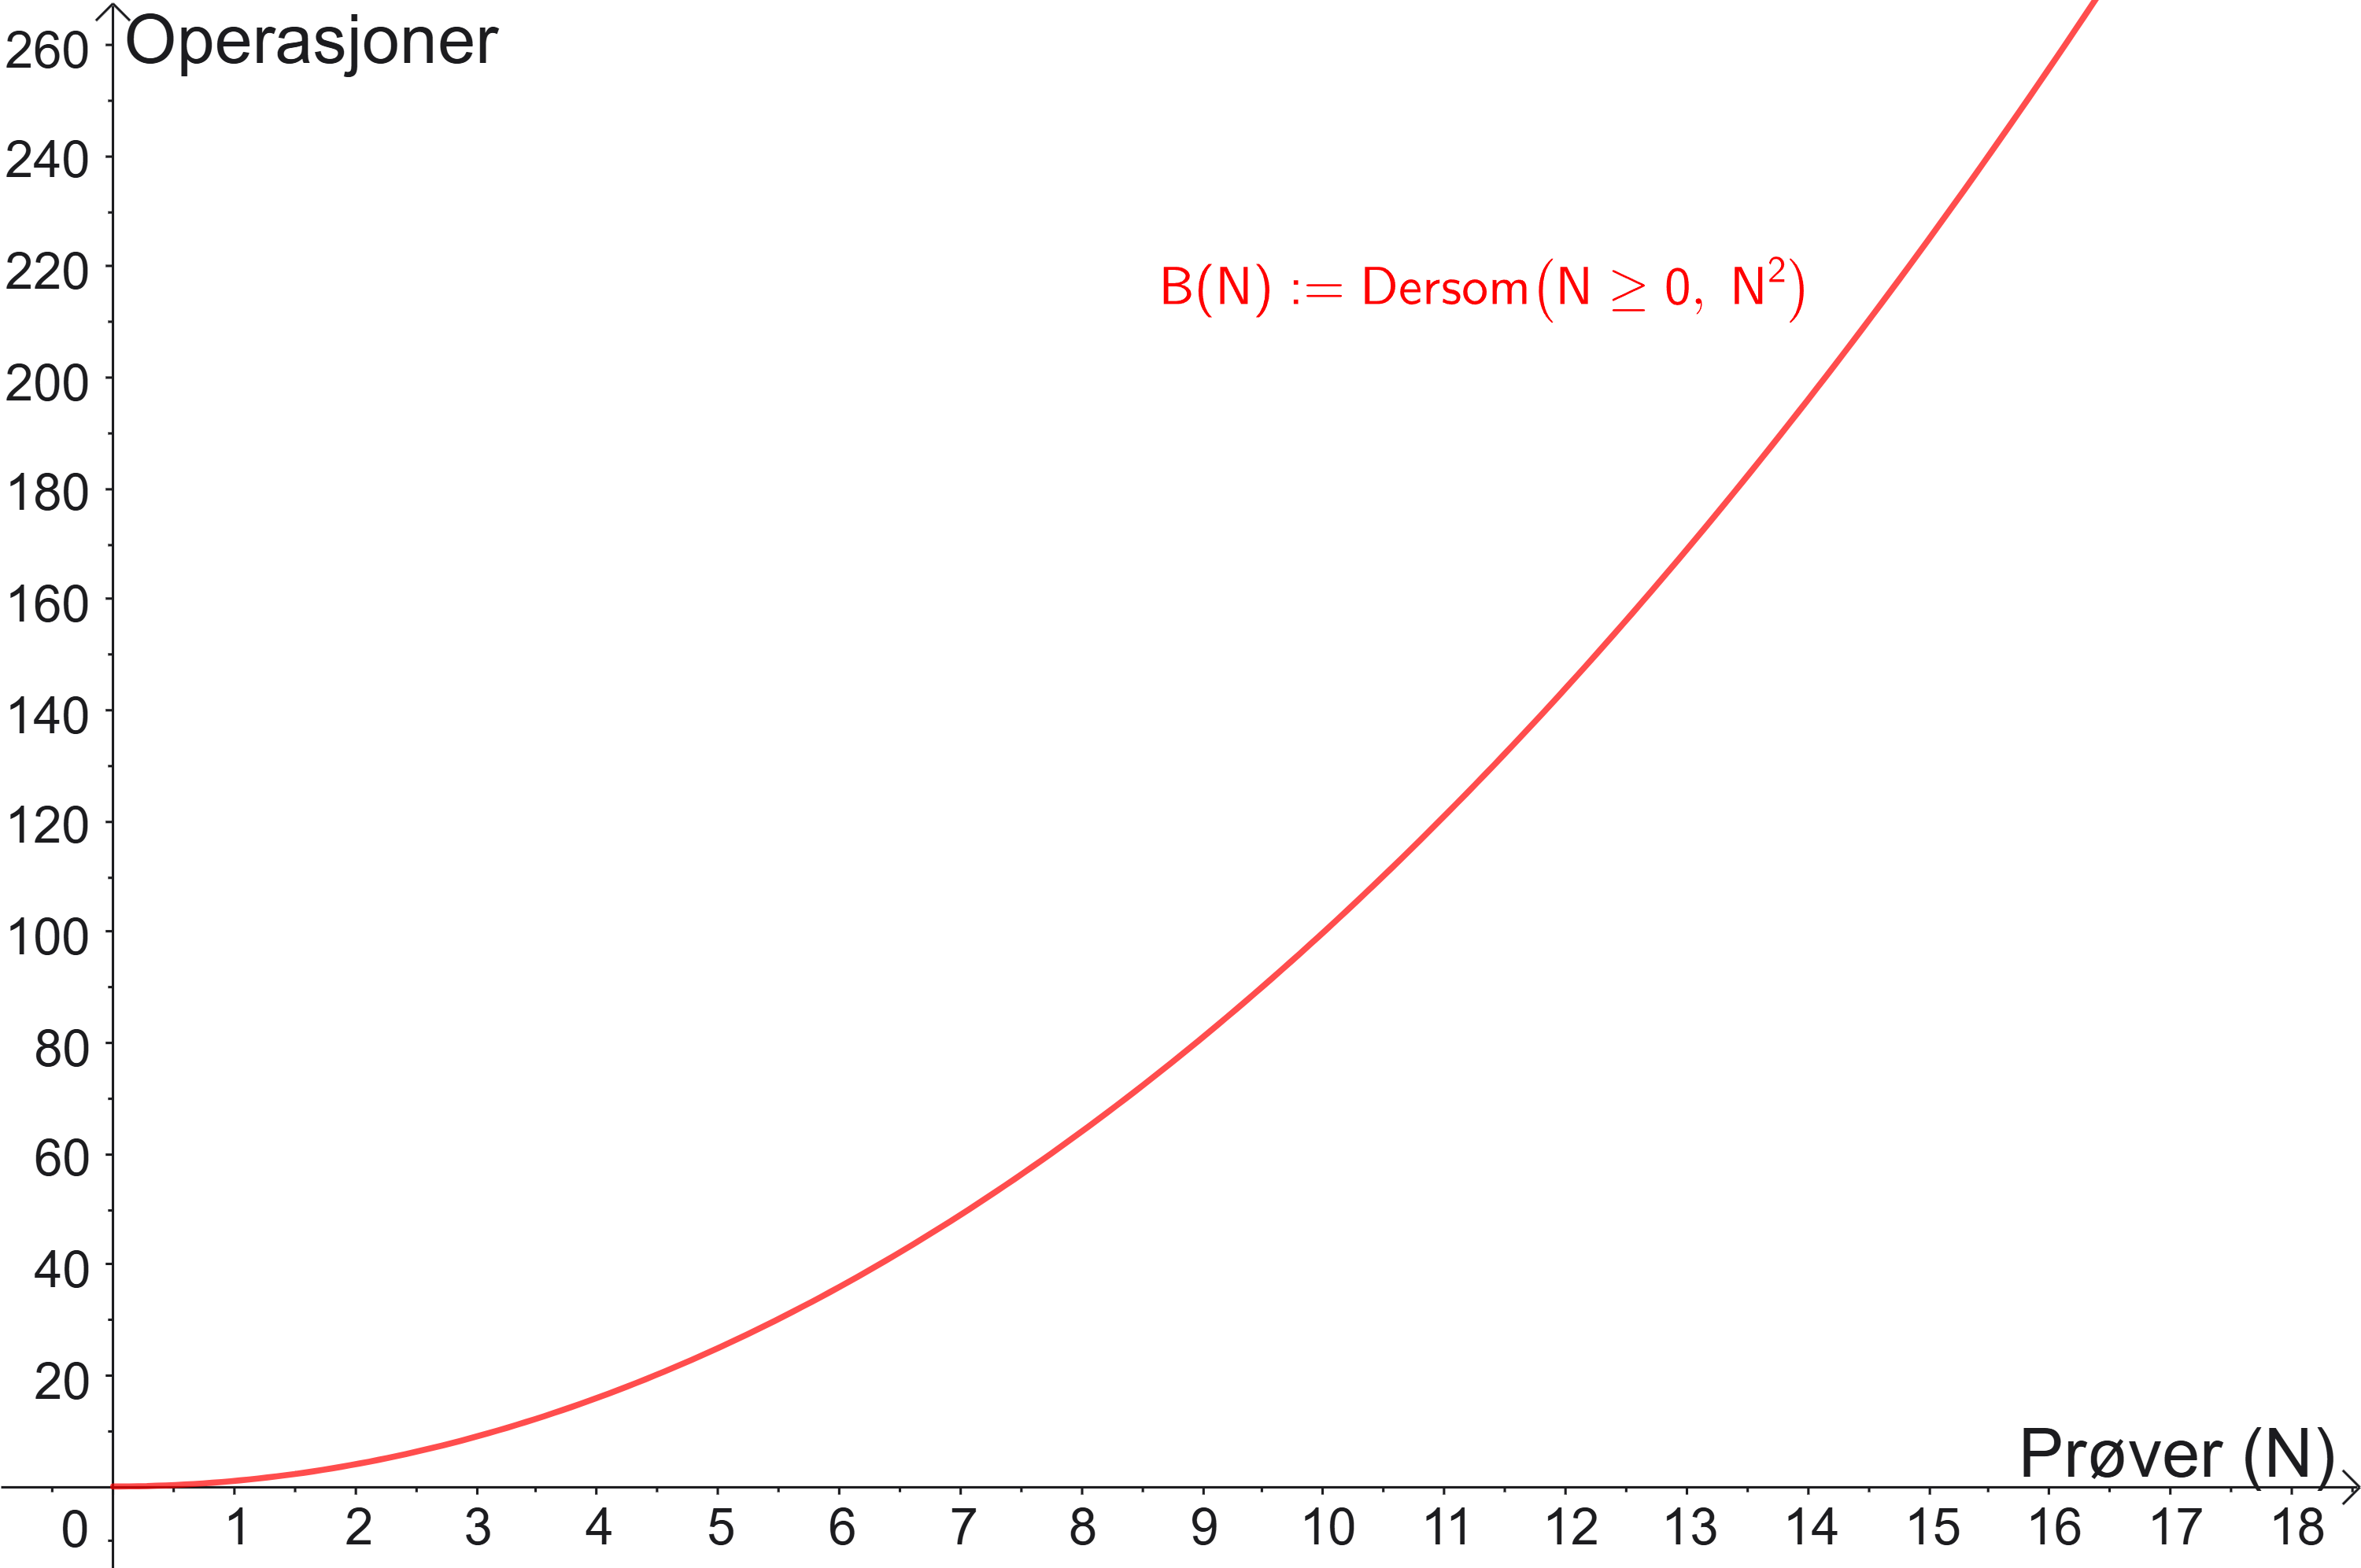
\includegraphics[width=0.8\textwidth]{./Media/DFT_Complexity.png}
    \caption{Beregningstid for DFT som funksjon av antall prøver $N$.}
    \label{fig:DFT_Complexity}
\end{figure}
\clearpage
\noindent
\subsection{Fast Fourier Transform (FFT)}
Som beskrevet tidligere har DFT en tidskompleksitet på $O(N^2)$, noe som kan være ineffektivt for lange signaler siden det tar lengre tid. For å løse dette problemet ble Fast Fourier Transform (FFT) utviklet. FFT er en familie av effektive algoritmer for å beregne DFT med betydelig redusert tidskompleksitet. Den reduserer tidskompleksiteten fra $O(N^2)$ til $O(N \log N)$ ved å utnytte symmetrier i DFT og dele opp beregningene i mindre deler. FFT er spesielt nyttig for lange signaler, der den betydelige reduksjonen i beregningstid kan være avgjørende for sanntidsapplikasjoner slik som lyd- og bildebehandling. Blant de mest kjente FFT-algoritmene er Cooley-Tukey-algoritmen (Radix-2), som vi skal bruke som et eksempel. Notasjonen vi bruker er formelen for DFT \eqref{DFT}:
\[
    X[k] = \sum_{n=0}^{N-1} x[n] W_{N}^{kn}, \quad W_{N} = e^{-\jj 2 \pi / N}
\]
Her bruker vi $W_{N}$ for å indikere $N$-punkt DFT. Denne kan deles opp i to summer, en for partallsindekserte elementer og en for oddetallsindekserte elementer:
\[
    X[k] = \sum_{m=0}^{N/2-1} x[2m] W_{N}^{k(2m)} + \sum_{m=0}^{N/2-1} x[2m+1] W_{N}^{k(2m+1)}
\]
Ved å faktorisere ut $W_{N}^{k}$ fra den andre summen får vi: 
\[
    X[k] = \sum_{m=0}^{N/2-1} x[2m] W_{N}^{2km} + W_{N}^{k} \sum_{m=0}^{N/2-1} x[2m+1] W_{N}^{2km}
\]
Legg merke til at:
\[
    W_{N}^{2km} = e^{-\jj 2 \pi (2km) / N} = e^{-\jj 2 \pi km / (N/2)} = W_{N/2}^{km}
\]
Som tilsvarer DFT av lengde $N/2$. Vi kan derfor definere to nye DFT-er:
\[
    E[k] = \sum_{m=0}^{N/2-1} x[2m] W_{N/2}^{km}, \quad O[k] = \sum_{m=0}^{N/2-1} x[2m+1] W_{N/2}^{km}
\]
Dermed kan vi skrive:
\[
    X[k] = E[k] + W_{N}^{k} O[k], \quad k = 0, 1, \ldots, N/2 - 1
\]
For $k = 0 \ldots N/2 - 1$ får vi også (pga periodisiteten til DFT):
\[
    X[k + N/2] = E[k] - W_{N}^{k} O[k], \quad k = 0, 1, \ldots, N/2 - 1
\]
Grunnen til at vi får minus-tegnet i den andre ligningen er at:
\[
    W_N^{k + N/2} = W_N^k \cdot W_N^{N/2} = W_N^k \cdot e^{-\jj \pi} = -W_N^k
\]
Vi har da butterfly-operasjonen:
\[
    X[k] = E[k] + W_{N}^{k} O[k], \qquad X[k + N/2] = E[k] - W_{N}^{k} O[k], \quad k = 0, 1, \ldots, N/2 - 1
\]
\clearpage
\noindent
Dette betyr at vi kan beregne en $N$-punkt DFT ved å beregne to $N/2$-punkt DFT-er, noe som reduserer antall nødvendige beregninger betydelig. Ved å gjenta denne prosessen rekursivt til vi når DFT-er av lengde 2, oppnår vi den effektive FFT-algoritmen med tidskompleksitet $O(N \log N)$. Dette kan vi se ved å la $B(N)$ være antall grunnoperasjoner for en $N$-punkts FFT. Da har vi:
\[
    B(N) = aB(N/b) + cN, \quad B(1) = c_0
\]
hvor $a$ er antall delproblemer (her $2$), $b$ er faktoren vi deler problemet med (her $2$), og $cN$ representerer den lineære tiden som kreves for å kombinere resultatene, $c$ er altså en konstant. Dette gir:
\[
    B(N) = 2B(N/2) + cN
\]
Siden $N=2^m$ har rekursjonstreet $m=\log_2 N$ nivåer. Hvert nivå koster lineær tid i $N$ (ca. $N/2$ \emph{butterflies}), vi får derfor totalt:
\textcolor{red}{Vis en figur som beskriver hva "butterflies" er}
\[
    B(N)=cN\log_2 N=O(N\log_2 N).
\]
Dette gjør FFT til en svært effektiv metode for å beregne DFT, spesielt for store datasett noe som er observerses ved å se på plottet i figur \ref{fig:DFT_Complexity}.
\begin{figure}[h]
    \centering
    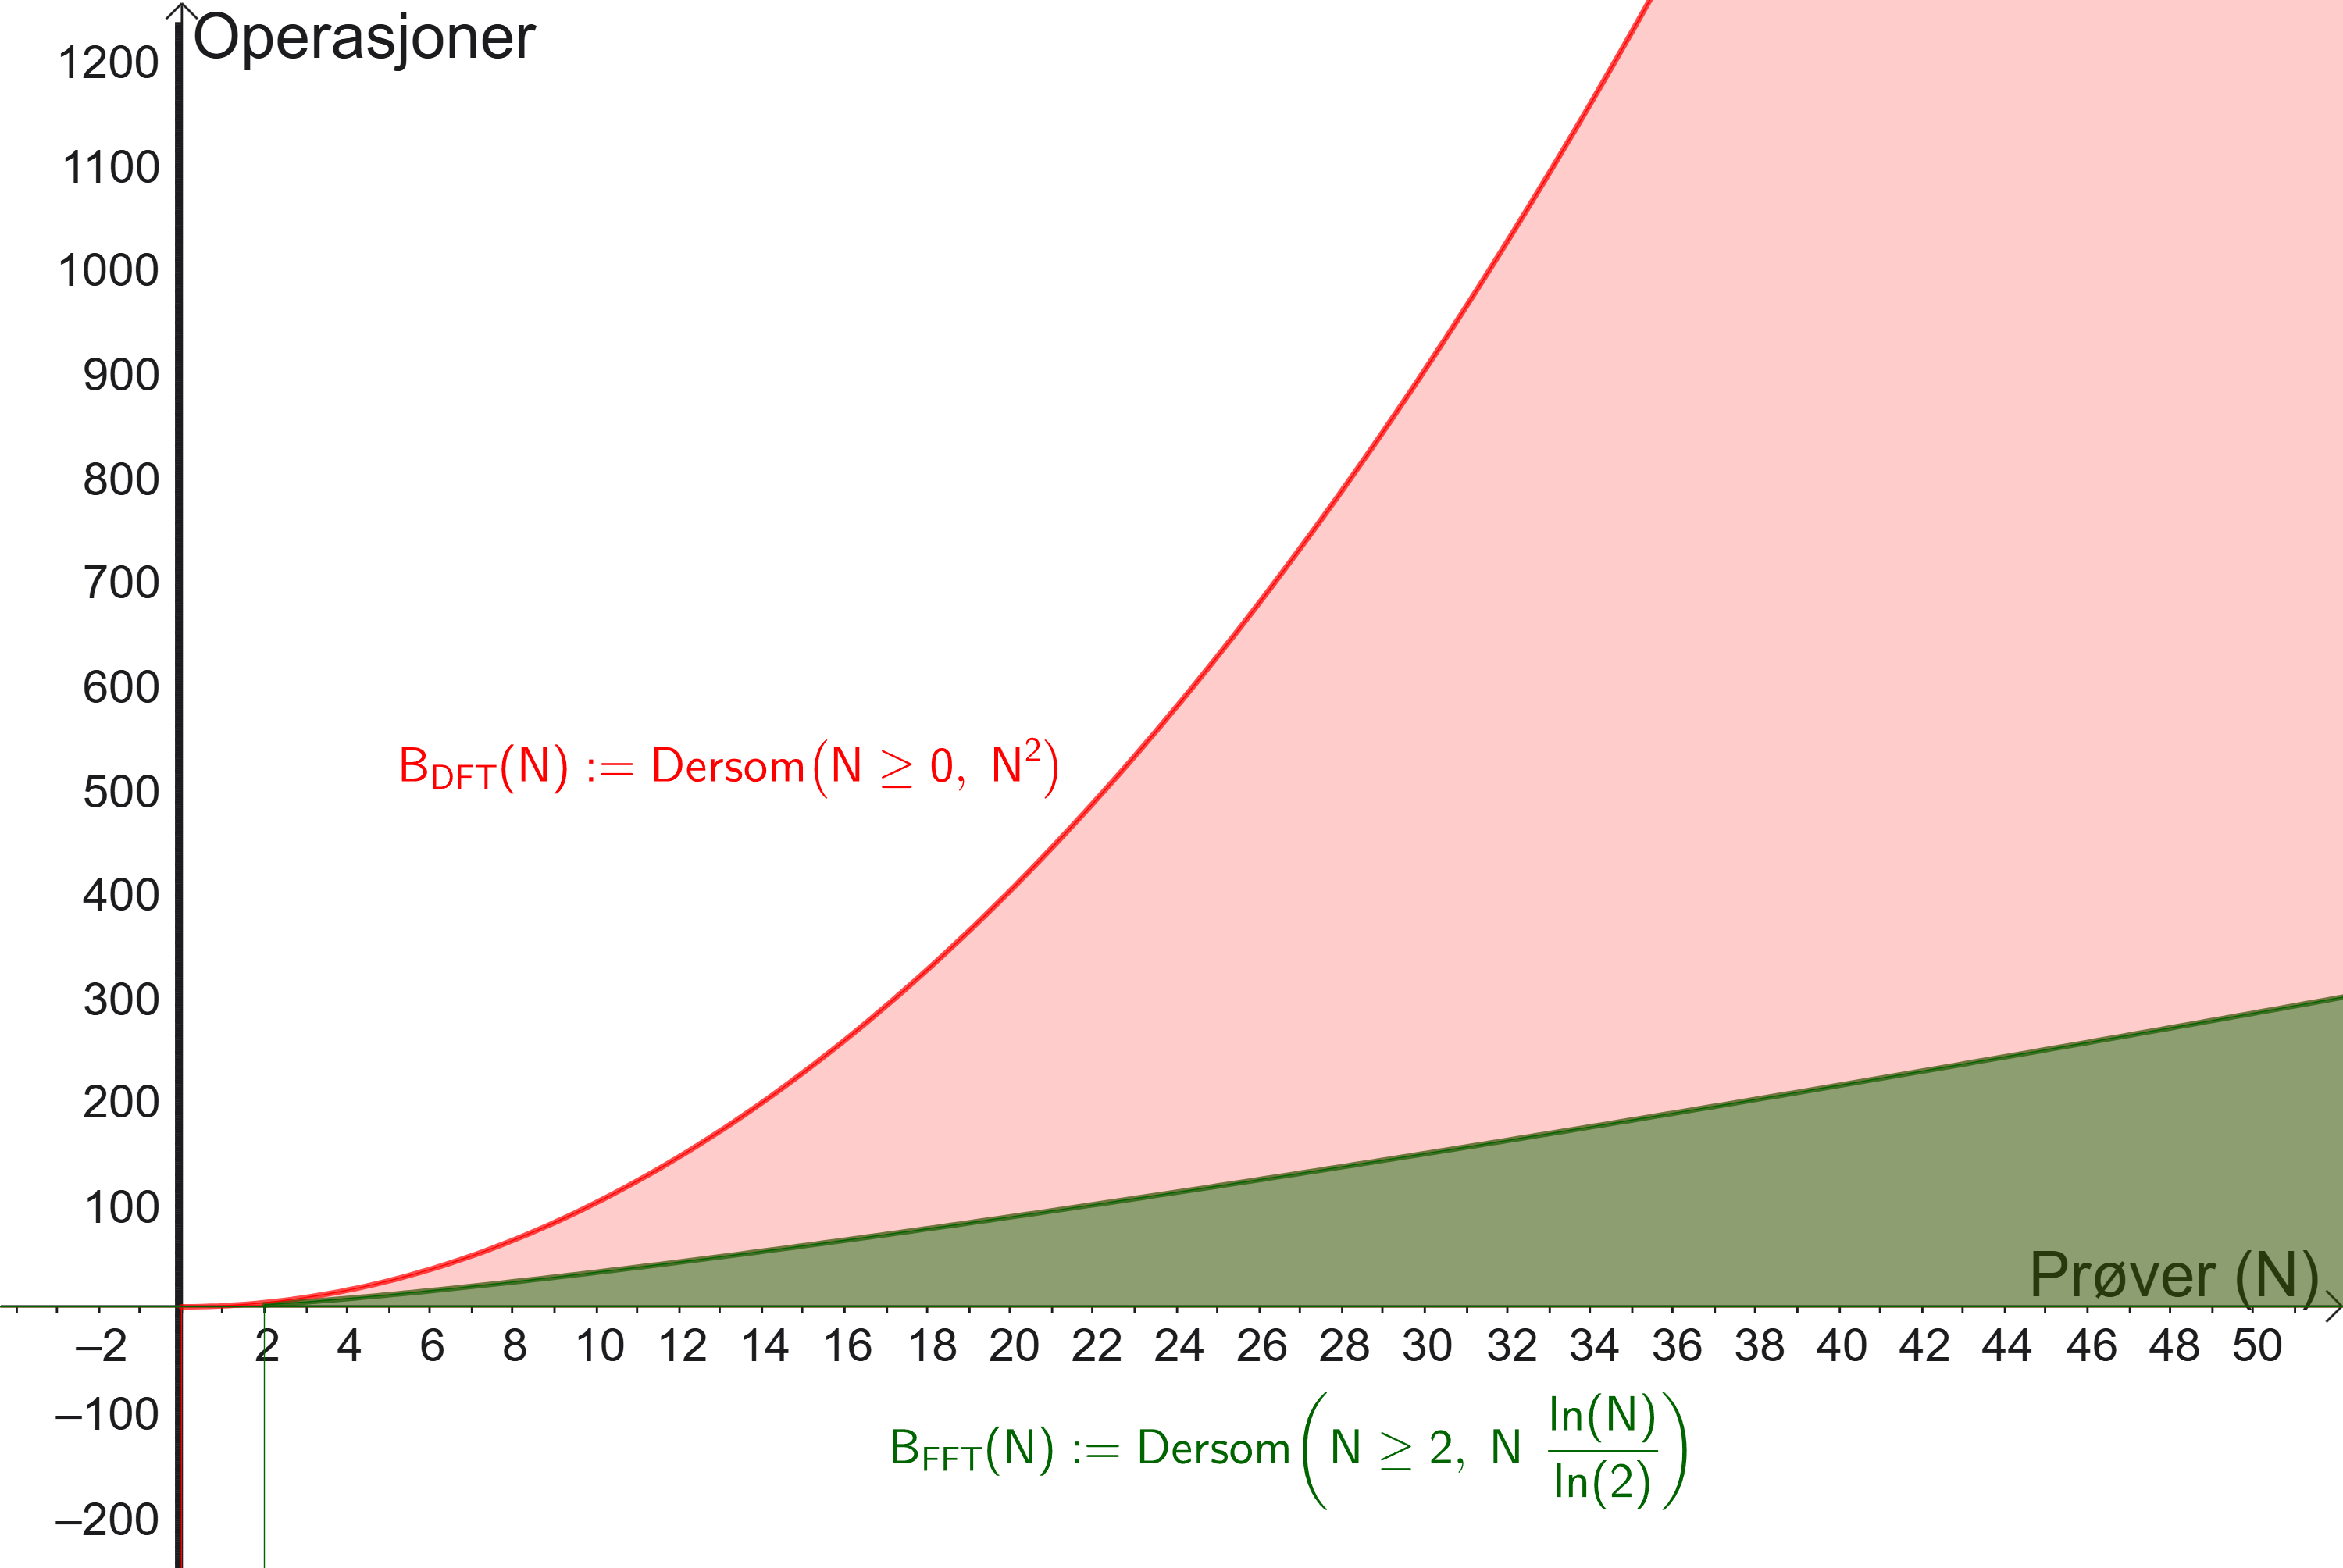
\includegraphics[width=.9\textwidth]{./Media/DFT_Complexity_VS_FFT.png}
    \caption{operasjoner for DFT vs FFT som funksjon av antall prøver $N$.}
    \label{fig:FFT_Complexity}
\end{figure}
\clearpage 
\noindent
\subsection{Short-Time Fourier Transform (STFT)}
STFT er en utvidelse av Fourier-transformasjonen som gjør det mulig å analysere tidsvarierende signaler. I stedet for å bruke hele signalet som inngang til DFT, deler STFT signalet opp i korte, overlappende segmenter (rammer) og beregner DFT for hvert ramme. Dette gir informasjon om hvordan frekvensinnholdet i signalet endres over tid. Matematisk kan STFT defineres som:
\[
    \text{STFT}\{x[n]\}(m, k) = \sum_{n=-\infty}^{\infty} x[n] w[n - mH] e^{-\jj 2 \pi k n / N}
\]
hvor \(w[n]\) er vindusfunksjonen, \(m\) er tidsindeksen for rammen, og \(k\) er frekvensindeksen. Ved å bruke STFT kan vi visualisere tids-frekvensrepresentasjonen av signalet, noe som er nyttig i mange applikasjoner som talegjenkjenning, musikkprosessering og mer.

\subsection{Fourier-transform kode i tonegjenkjenning}

\subsubsection{Vindusfunksjoner (Windowing)}
Fourier-transform innebærer å analysere et kontinuerlig signal som er på formen:
\[
x(t): \mathbb{R} \rightarrow \mathbb{R}
\]

\noindent
I praksis kan imidlertid lydsignaler ikke analyseres som uendelige kontinuerlige signaler, siden de er tidsvarierende. 
For å kunne anvende Fourier-transformasjonen deler man derfor signalet opp i mindre segmenter (vinduer), der hvert vindu antas å være tilnærmet stasjonært. 
På denne måten kan man finne hvilke frekvenser som er tilstede i et gitt tidsintervall $\Delta t$ [s]. \\

Vindusfunksjonen vekter signalet før transformasjonen og demper amplituden mot kantene av vinduet. 
Dette gjør at signalet går gradvis mot null ved start og slutt, noe som gir en jevnere overgang mellom vinduene og reduserer såkalt \textit{spectral leakage}. 
Dermed blir frekvensanalysen mer presis. 

\textbf{Hanning-vinduet} er en vanlig vindusfunksjon og brukes også i vårt prosjekt. Den er definert som:

\begin{equation}
    w[n]=\frac{1}{2} \left( 1 - \cos{\left( \frac{2 \pi n}{N - 1}\right)} \right)
    \label{eq:HanningVinduFunksjon}
\end{equation}

\noindent
der $N$ er antall prøver i vinduet. 
Hanning-vinduet gir en god balanse mellom frekvensoppløsning og lekkasjereduksjon. 
I koden multipliseres hvert signalutdrag med et Hanning-vindu før FFT-beregningen, slik at de beregnede frekvenskomponentene bedre representerer de faktiske tonene i lyden vi analyserer. Grafen under viser hvordan et signal $x[t]$ hvis vi bruker en Hanning-vindu transformasjon på signalet:

\begin{figure}[h!]
    \centering
    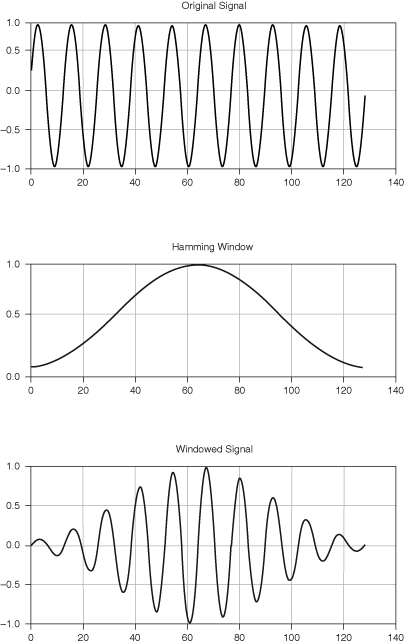
\includegraphics[width=0.4\textwidth]{./Media/hanningVinduGrafikk.png}
    \caption{Hanning-vinduet på et signal}
    \label{fig:HanningVinduGraf}
\end{figure}

\subsubsection{Parabolsk toppinterpolasjon (Quadratic interpolation)}
FFT gir diskrete frekvenspunkter, men den faktiske tonen kan ligge mellom disse frekvenspunktene. Interpolasjon kan benyttes for å bedre presisjonen for analysen. Denne interpolasjonen kan oppnås ved bruk av parabolsk toppinterpolasjon. Uten interpolasjon får vi kun en oppløsning gitt ved
\[
\Delta f = \frac{f_s}{N}
\]

\noindent
der $f_s$ er samplingsfrekvensen og $N$ er antall FFT diskrete frekvenspunkter.

\subsubsection{Frekvens-til-note konvertering (Pitch Mapping)}





\subsection{Root Mean Square (RMS)}
RMS er nyttig når man skal måle eller sammenligne styrken til et signal over tid. Det brukes også i støyanalyse for å finne et representativt “gjennomsnittsnivå” av lydintensiteten. RMS gir et mål på den \textbf{effektive verdien av amplituden} til et signal, og gir dermed et bedre bilde av den \textbf{opplevde energien i lyden} enn et vanlig gjennomsnitt.

Matematisk defineres RMS for et diskret signal $x[n]$ med $N$ prøver som:
\begin{equation}
    x_{RMS} = \sqrt{\frac{1}{N} \sum_{n=1}^{N} x[n]^2}
    \label{eq:RMS}
\end{equation}
\noindent
Matematisk ser vi at beregningen innebærer å kvadrere hver verdi av $x[n]$ for å gjøre alle amplituder positive, deretter tar gjennomsnittet og til slutt roten av resultatet. RMS kan brukes til å måle lydnivået over tid, sammenligne styrken til ulike signaler og redusere støy. \\
I kombinasjon med Fourier-transformasjonen og tonegjenkjenning kan RMS brukes for å evaluere energinivået innenfor bestemte frekvensområder. Det betyr at vi kan identifisere hvilken frekvens som har høyest RMS verdi og determinere hovedtonen i et signal.

\subsubsection{Støydemping i kode (støygating)}
For å redusere påvirkningen av bakgrunnsstøy brukes en enkel RMS-basert støygate. Ved hver FFt-beregning estimeres energien i vinduet med hjelp av den matematiske definisjonen for RMS (Ligning (\ref{eq:RMS})). En glattet støyterskel beregnes kontinuerlig ved hjelp av en eksponentiell glatting:
\[
\text{noise}_{t+1} = \alpha \cdot \text{noise}_t + (1 - \alpha) \cdot x_{\text{RMS}}
\]
der $\alpha$ er en glattefaktor mellom 0 og 1. 
Dersom den aktuelle RMS-verdien i vinduet er lavere enn en gitt multiplikator av støyterskelen, ignoreres vinduet:
\[
\text{hvis } x_{\text{RMS}} < \text{noise\_multiplier} \cdot \text{noise}, \text{ hopp over analysen.}
\]
Denne metoden kalles \textbf{RMS-gating} og hindrer at bakgrunnsstøy og lavintensive signaler analyseres som gyldige toner.